\documentclass[8pt]{beamer}
\usepackage{tikz}
\usepackage[utf8]{vietnam}
\usepackage{amsmath}
\usepackage{graphicx}
\usepackage{mathrsfs}
\usepackage{amssymb,amsfonts,amsthm}
\usepackage{wrapfig}
\usepackage{hyperref}
\usetheme{Copenhagen}
\usecolortheme{spruce}
\setbeamertemplate{navigation symbols}{}
\setbeamertemplate{headline}{}
\setbeamertemplate{footline}{}
\title[Kết quả nghiên cứu tuần 1]
{Kết quả nghiên cứu tuần $1$}
\subtitle{Phòng thí nghiệm Thông tin Vô tuyến}
\author[Phòng thí nghiệm thông tin Vô tuyến]
{Tín Vũ}
\date[VLC 2021] % (optional)
{tinvu1309@gmail.com}
\begin{document}
\frame{\titlepage}
\begin{frame}{Mục lục}
\tableofcontents
\end{frame}
\begin{frame}{Tài liệu tham khảo}
\section{Tài liệu tham khảo}
Tài liệu tham khảo được sử dụng để nghiên cứu gồm: Calculus 7E (James Stewart), Antenna Theory (A.Balanis).
\end{frame}
\begin{frame}{Các kết quả cơ bản}
\section{Các kết quả cơ bản}
\begin{itemize}
\item Tích phân đường
\end{itemize}
\subsection{Tích phân đường}
\subsubsection{Tích phân đường vô hướng}
\begin{itemize}
	\item[-] Tích phân đường vô hướng
\end{itemize}
\begin{figure}[h]
			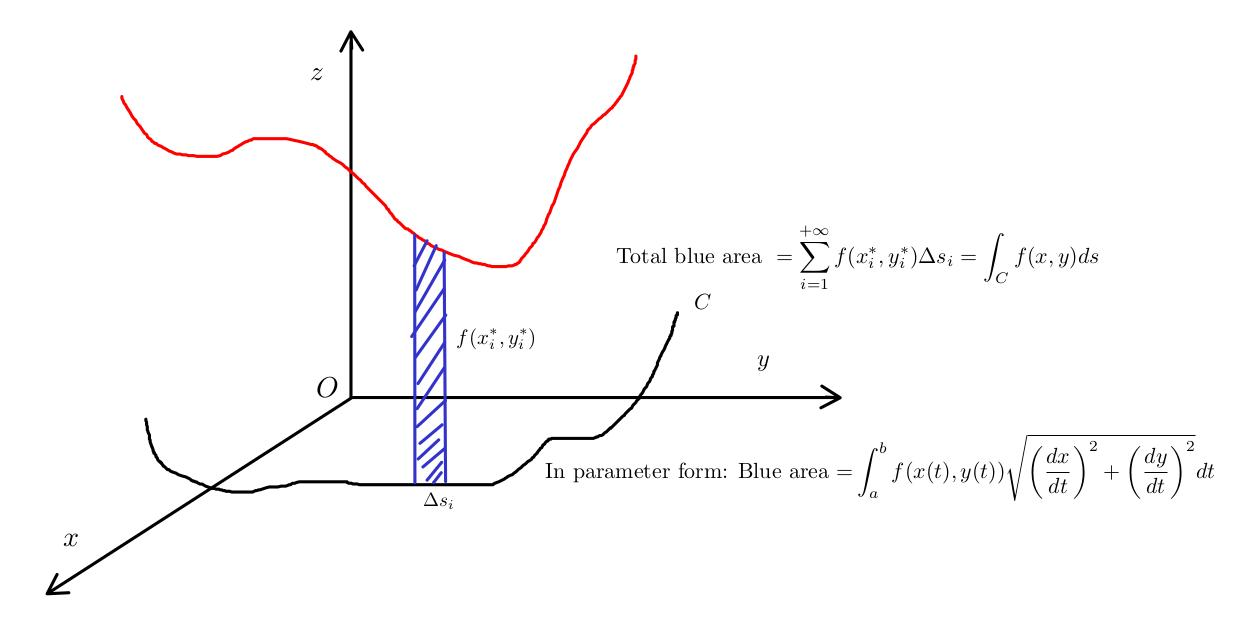
\includegraphics[width=0.9\textwidth]{line.jpg}
			\caption{Scalar line integral}			\label{fig:re1}
\end{figure}
\end{frame}
\begin{frame}{Các kết quả cơ bản}
\begin{itemize}
	\item[-] Tích phân đường có hướng
\end{itemize}
\subsubsection{Tích phân đường có hướng}
\begin{figure}[h]
			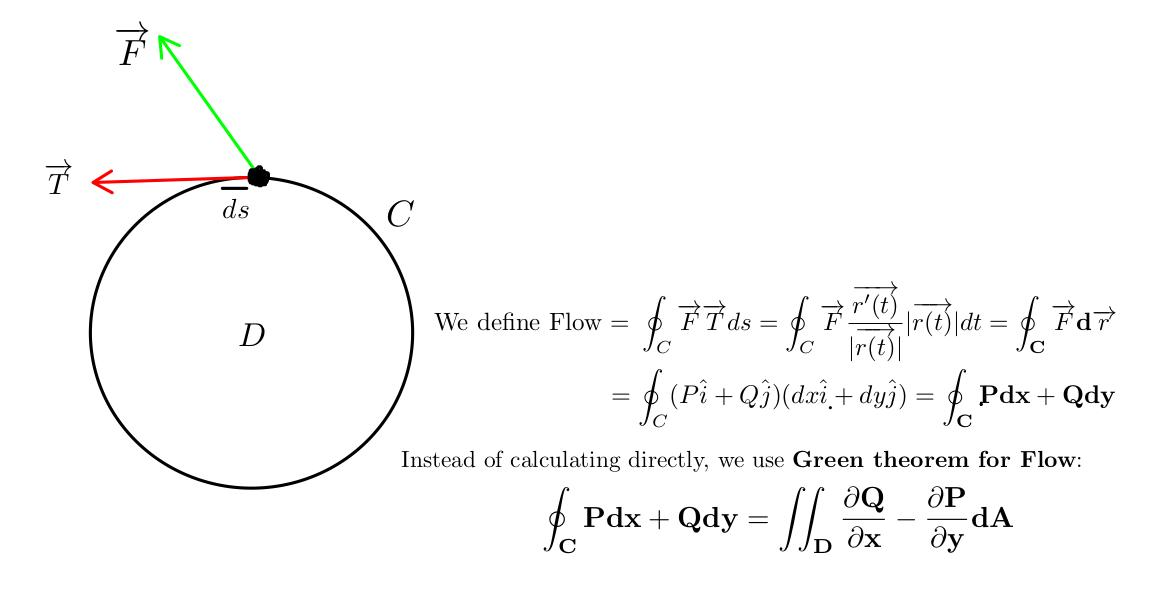
\includegraphics[width=1\textwidth]{green1.jpg}
			\caption{Green's theorem for Flow}			\label{fig:re2}
\end{figure}

\end{frame}
\begin{frame}{Các kết quả cơ bản}
Chúng ta sẽ chứng minh lại định lý Green cho trường hợp đơn giản nhất, xét đường đơn liên kín C như hình vẽ sau:
\begin{figure}[h]
			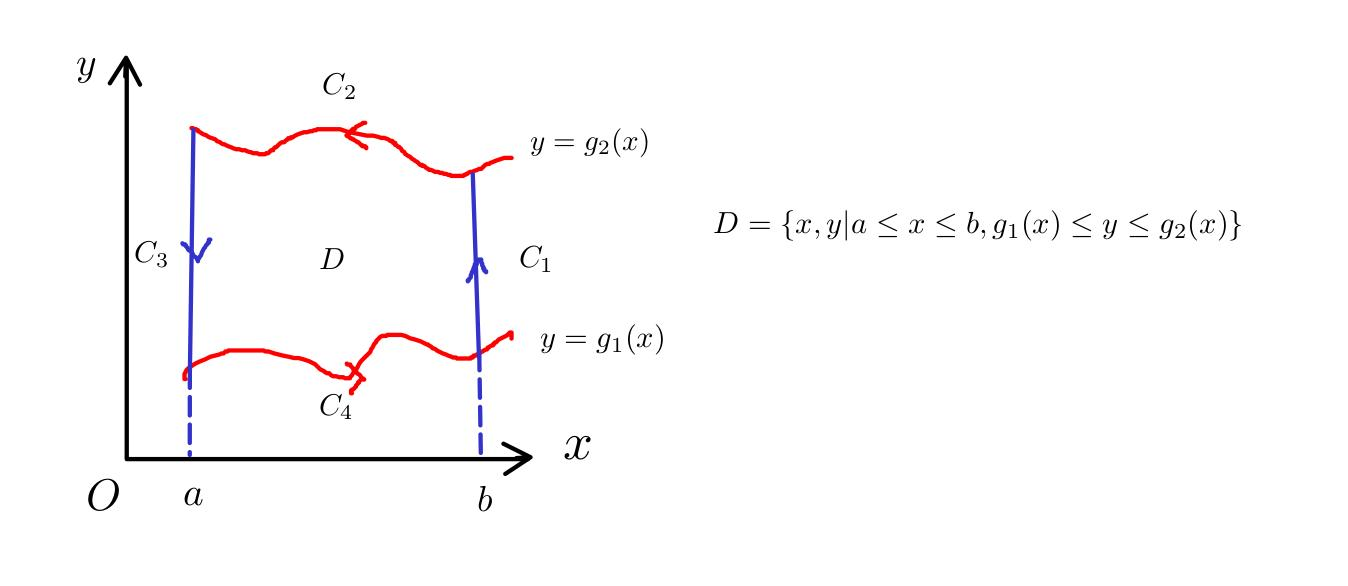
\includegraphics[width=0.9\textwidth]{domain.jpg}
			\caption{Proof of Green's theorem for Flow}			\label{fig:re3}
\end{figure}
Để cho đơn giản, ta chỉ chứng minh đẳng thức: $$\oint_{C}Pdx=-\iint_{D}\frac{\partial P}{\partial y}dA$$
\end{frame}
\begin{frame}{Các kết quả cơ bản}
\begin{equation*}
\begin{split}
	\oint_{C}Pdx &=\int_{a}^{b}P(x,g_{1}(x))+\int_{b}^{a}P(x,g_{2}(x))dx=\int_{a}^{b}P(x,g_{1}(x))dx-\int_{a}^{b}P(x,g_{2}(x))dx\\
	\iint_{D}\frac{\partial P}{\partial y}dA &=\int_{a}^{b}\int_{g_{1}(x)}^{g_{2}(x)}\frac{\partial P}{\partial y}dydx=\int_{a}^{b}P(x,g_{2}(x))dx-\int_{a}^{b}P(x,g_{1}(x))dx\\
						 &\Rightarrow\oint_{C}Pdx=-\iint_{D}\frac{\partial P}{\partial y}dA
\end{split}
\end{equation*}
Chứng minh tương tự, ta cũng thu được $$\oint_{C}Qdy=\iint_{D}\frac{\partial Q}{\partial x}dA\Rightarrow \oint_{C}Pdx+Qdy=\iint_{D}\left(\frac{\partial Q}{\partial x}-\frac{\partial P}{\partial y}\right)dA$$
Ta viết lại công thức Green dạng \textbf{curl}:
$$\oint_{C}Pdx+Qdy=\iint_{D}\textbf{curl}\overrightarrow{F}\hat kdA=\iint_{D}(\nabla \times \overrightarrow{F})\hat kdA$$
\end{frame}
\begin{frame}{Các kết quả cơ bản}
\begin{figure}[h]
			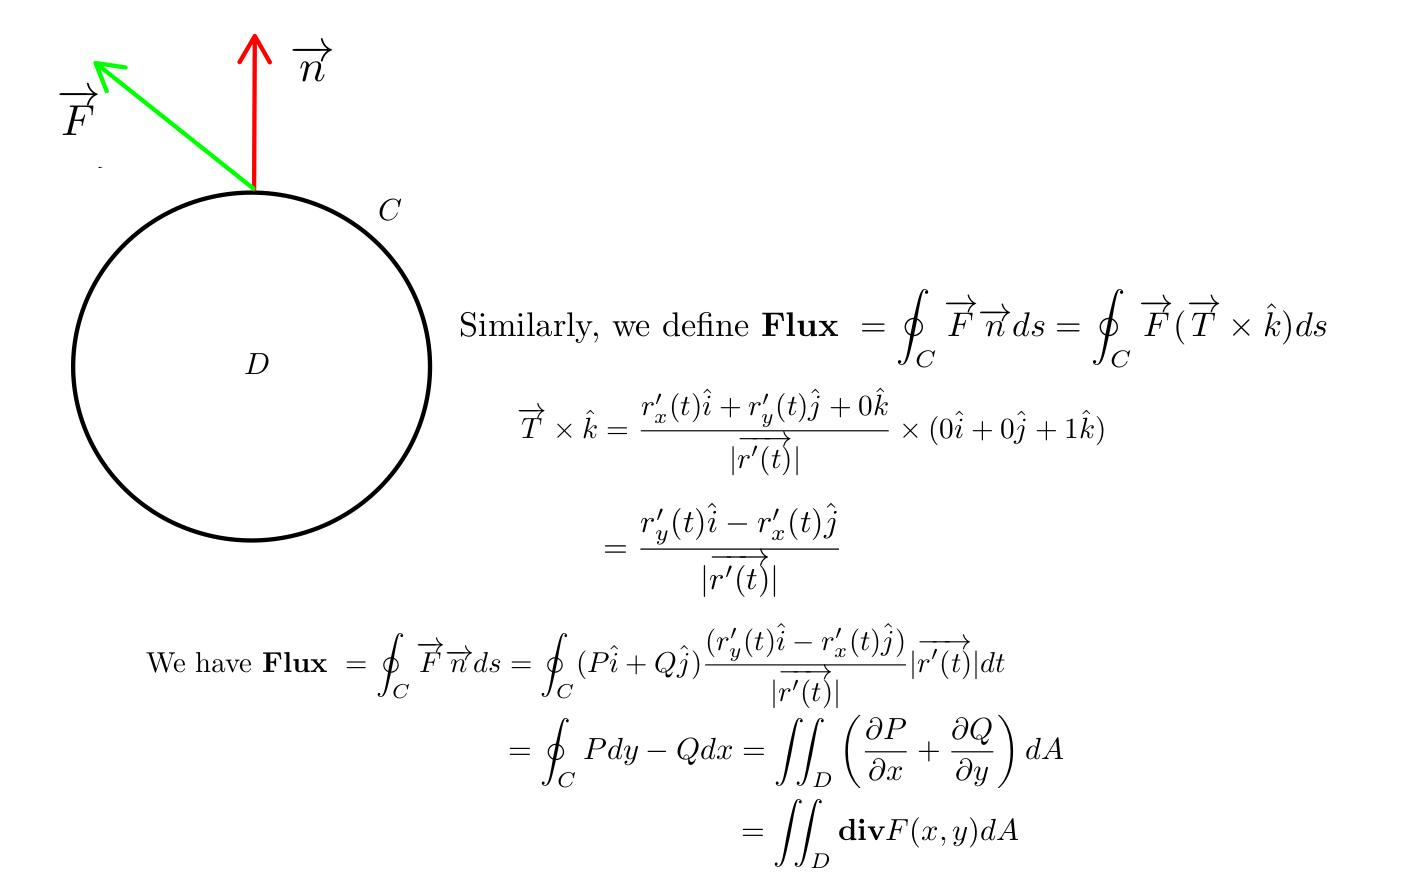
\includegraphics[width=1\textwidth]{flux.jpg}
			\caption{Green's theorem for Flux}			\label{fig:re4}
\end{figure}

\end{frame}
\begin{frame}{Các kết quả cơ bản}
\subsection{Tích phân mặt}
\subsubsection{Diện tích mặt}

\begin{itemize}
	\item Diện tích mặt
\end{itemize}
Mọi mặt phẳng bất kì đều có thể được biểu diễn rất dễ dàng qua hàm vector $$\overrightarrow{r(u,v)}=x(u,v)\hat i+y(u,v)\hat j+z(u,v)\hat k$$
Ta xét một mặt bất kì được biểu diễn bởi hàm vector trên, với $(u,v)\in D$, ta muốn tìm diện tích mặt này.
\begin{figure}[h]
			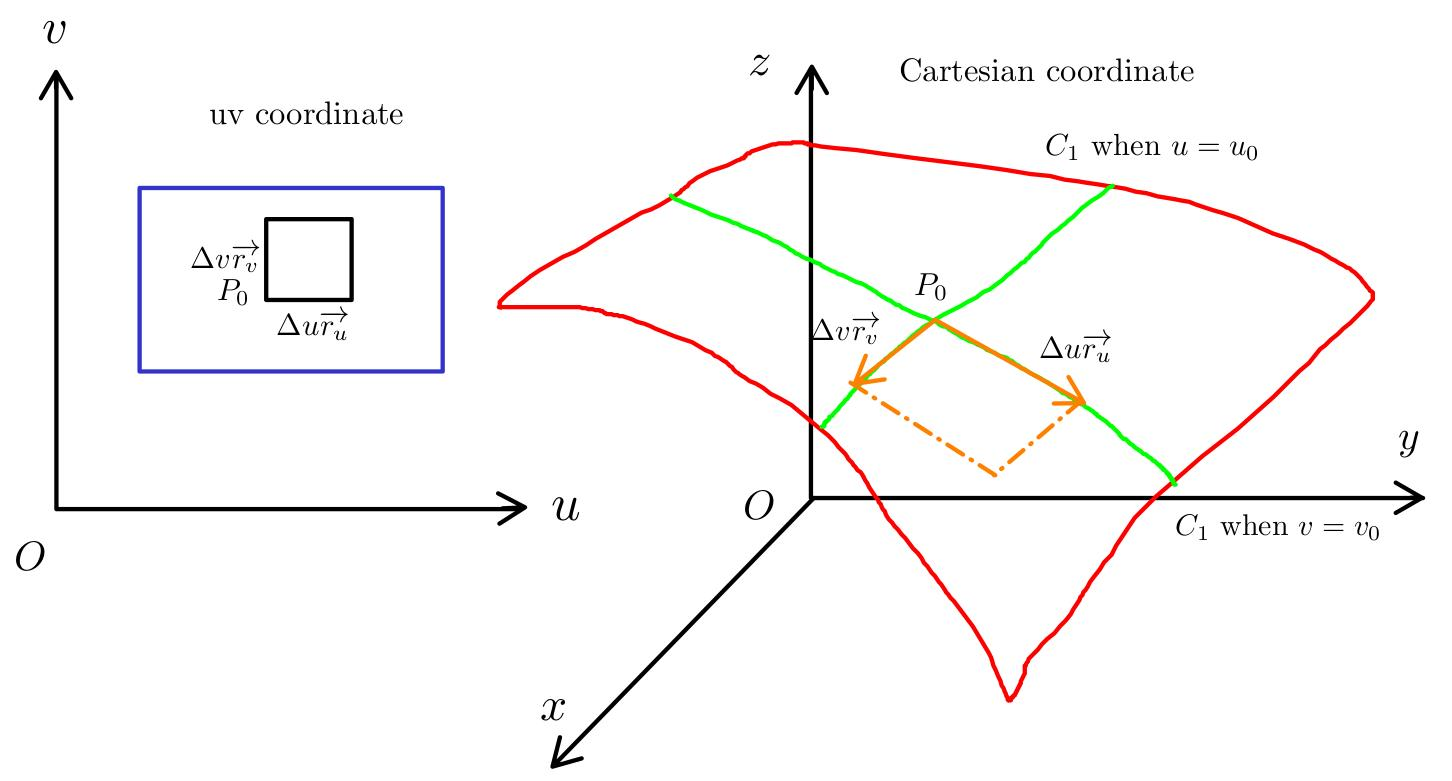
\includegraphics[width=0.8\textwidth]{cartesina.jpg}
			\caption{Surface Area}			\label{fig:re4}
\end{figure}
\end{frame}
\begin{frame}{Các kết quả cơ bản}
	Như đã thảo luận ở slide trước, ta có thể dễ dàng thấy rằng $\overrightarrow{r_{u}}$, $\overrightarrow{r_{v}}$ chính là 2 vector đạo hàm riêng lần lượt của biến $u$ và $v$. Đây chính là cặp vector tiếp tuyến của các đường cong $C_{1}$ và $C_{2}$ (đã chứng minh ở slide trước), với:
\begin{equation*}
\begin{split}
	\overrightarrow{r_{u}}&=\frac{\partial x(u,v)}{\partial u}\hat i+\frac{\partial y(u,v)}{\partial u}\hat j+\frac{\partial z(u,v)}{\partial u}\hat k
\end{split}
\end{equation*}

\begin{equation*}
\begin{split}
	\overrightarrow{r_{v}}&=\frac{\partial x(u,v)}{\partial v}\hat i+\frac{\partial y(u,v)}{\partial v}\hat j+\frac{\partial z(u,v)}{\partial v}\hat k
\end{split}
\end{equation*}
Ta có thể ước lượng xấp xỉ vi phân diện tích một mặt chữ nhật rất nhỏ:
$$dA(S)=|\overrightarrow{(r_{u}}du)\times(\overrightarrow{r_{v}}dv)|=|\overrightarrow{r_{u}}\times\overrightarrow{r_{v}}|dA$$
Vậy ta thu được diện tích toàn bộ mặt phẳng có thể được biểu diễn bằng tổng Riemann trực tiếp, ta viết lại đơn giản hơn như sau:
$$\alert{A(S)=\sum_{i=1}^{m}\sum_{j=1}^{n}|\overrightarrow{r_{u}}\times\overrightarrow{r_{v}}|=\iint_{D}|\overrightarrow{r_{u}}\times\overrightarrow{r_{v}}|dA}$$
Đây là kết quả cực kì quan trọng, sẽ liên tục được sử dụng trong phần tích phân mặt.
\end{frame}
\begin{frame}{Các kết quả cơ bản}
\begin{itemize}
	\item Tích phân mặt vô hướng
\end{itemize}
\subsubsection{Tích phân mặt vô hướng}
\begin{figure}[h]
			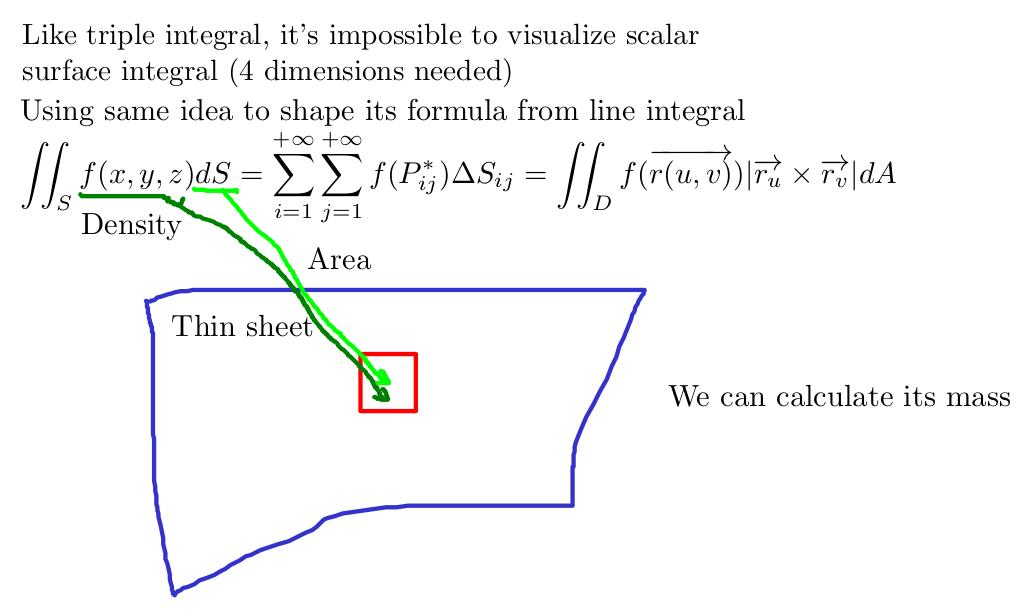
\includegraphics[width=0.9\textwidth]{sheet.jpg}
			\caption{Scalar surface integral}			\label{fig:re5}
\end{figure}

\end{frame}
\begin{frame}{Các kết quả cơ bản}
\subsubsection{Tích phân mặt có hướng}
\begin{itemize}
	\item Tích phân mặt có hướng
\end{itemize}
\begin{figure}[h]
			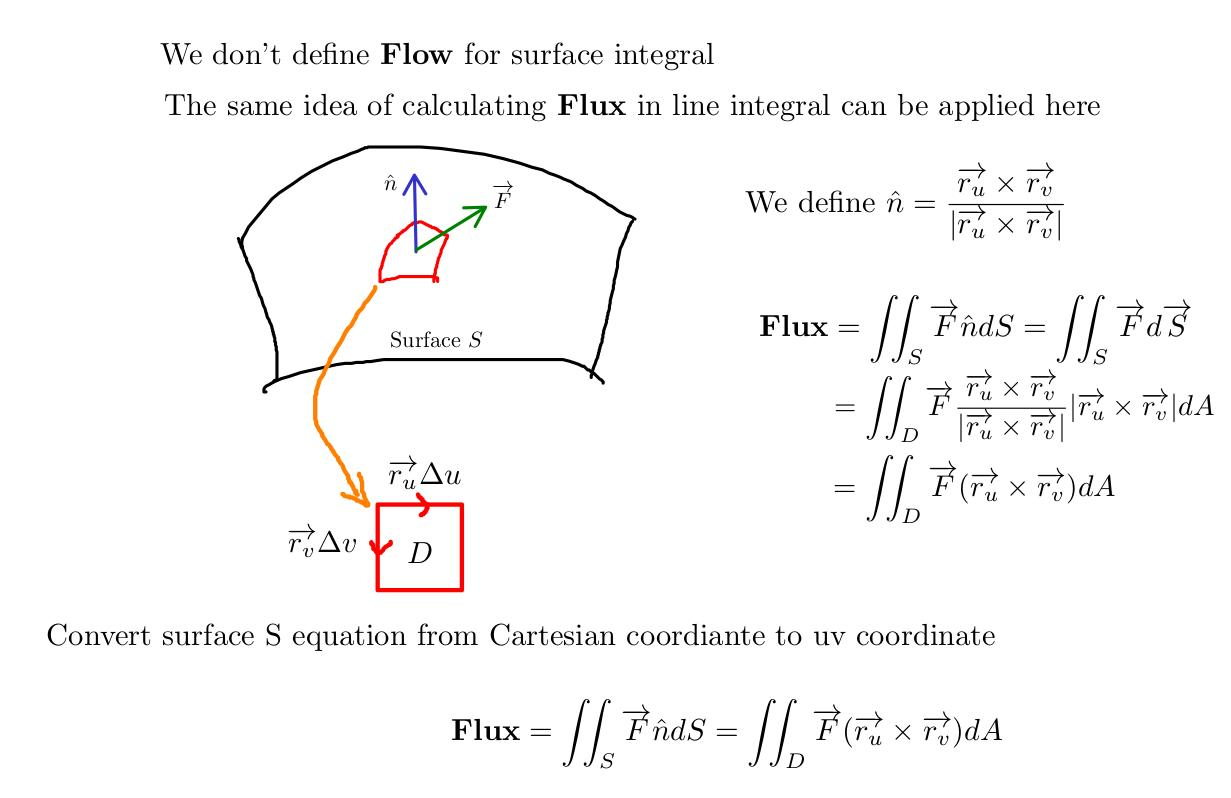
\includegraphics[width=0.9\textwidth]{fluxo.jpg}
			\caption{Flux in surface integral}			\label{fig:re5}
\end{figure}

\end{frame}
\begin{frame}{Các kết quả cơ bản}
Chúng ta tổng quát hóa định lý Green cho \textbf{Flux} và \textbf{Flow} trong không gian 3 chiều:
\begin{block}{Định lý Green trong không gian 2 chiều}
	\begin{equation*}
		\begin{split}
			\textbf{Flux}&=\oint_{C}\overrightarrow{F}\overrightarrow{n}ds=\iint_{D}\textbf{div}\overrightarrow{F}dA=\iint_{D}\nabla\cdot \overrightarrow{F}dA \\
			\textbf{Flow}&=\oint_{C}\overrightarrow{F}\overrightarrow{T}ds=\iint_{D}\textbf{curl}\overrightarrow{F}\hat k dA=\iint_{D}(\nabla\times\overrightarrow{F})\hat k dA
		\end{split}
	\end{equation*}
\end{block}
\begin{block}{Định lý Green trong không gian 3 chiều}
\begin{itemize}
	\item  Định lý phân kỳ (divergence theorem):$$\textbf{Flux}=\iint_{S}\overrightarrow{F}\hat n dS=\iint_{S}\overrightarrow{F}d\overrightarrow{S}=\iiint_{E}\textbf{div}\overrightarrow{F}dV$$
	\item Định lý Stoke: $$\textbf{Flow}=\int_{C}\overrightarrow{F}\overrightarrow{T}dS=\iint_{S}\textbf{curl}\overrightarrow{F}d\overrightarrow{S}$$
\end{itemize}
\end{block}
\end{frame}
\begin{frame}{}
\end{frame}
\end{document}

